\section{Sprzedaż}
Sprzedawca pośredniczy w kontaktach z kontrahentem i zarządza procesem
sprzedaży towarów. Przyjmuje on zamówienia (wykonuje operacje wydania
towaru z magazynu) i dodaje je do bazy, aktualizując jednocześnie dane
klientów. Sprawuje kontrolę nad realizacją wydania towaru z magazynu,
a w razie potrzeby może przyjąć zwrócony towar. Do zadań sprzedawcy
należy prowadzenie ewidencji kontrahentów, aktualizowanie informacji o
nich oraz usuwanie starych. Przypadki użycia sprzedawcy zostały
zaprezentowane na diagramie \ref{fig:Sprzedaz}.

\begin{figure}[H]
  \centering
  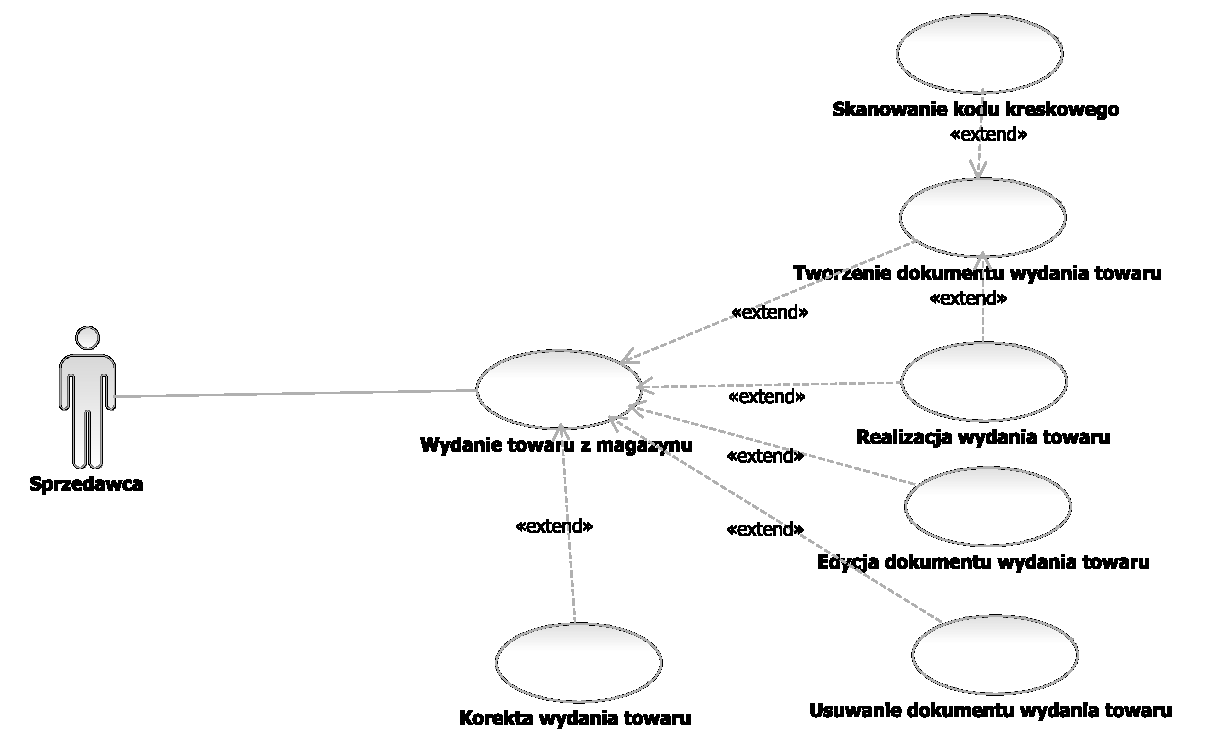
\includegraphics[scale=0.6]{../img/usecase/Sprzedaz.pdf}
  \caption{Diagram przypadków użycia dla sprzedaży.}
  \label{fig:Sprzedaz}
\end{figure}

\newpage
\singlespacing
\subsection{Wydanie towaru z magazynu}
\begin{usecase}
  \addtitle{PU12}{Wydanie towaru z magazynu}
  \addfield{Priorytet:}{wysoki}
  \addfield{Aktor główny:}{Sprzedawca}
  \addfield{Warunki początkowe:}{Aktor został uwierzytelniony.}
  % Warunki końcowe (brak).
  \addscenario{Scenariusz główny:}{
  \item Aktor wybiera opcję wydania towaru z magazynu.
  \item System wyświetla listę dokumentów WZ wraz z opcjami do zarządzania dokumentami wydania towaru.
  }
  \addfield{Wymagania funkcjonalne:}{5.}
\end{usecase}

\begin{figure}[H]
  \centering
  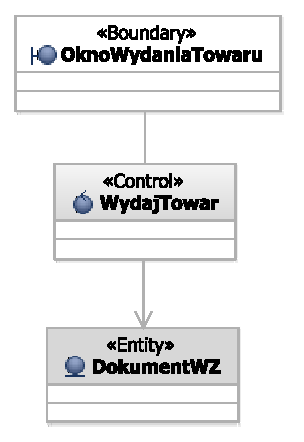
\includegraphics[angle=\ecbangle, scale=\ecbscale]{../img/usecase/pu12ecb.pdf}
  \caption{\ecbcaption12}
\end{figure}
\newpage
\begin{figure}[H]
  \centering
  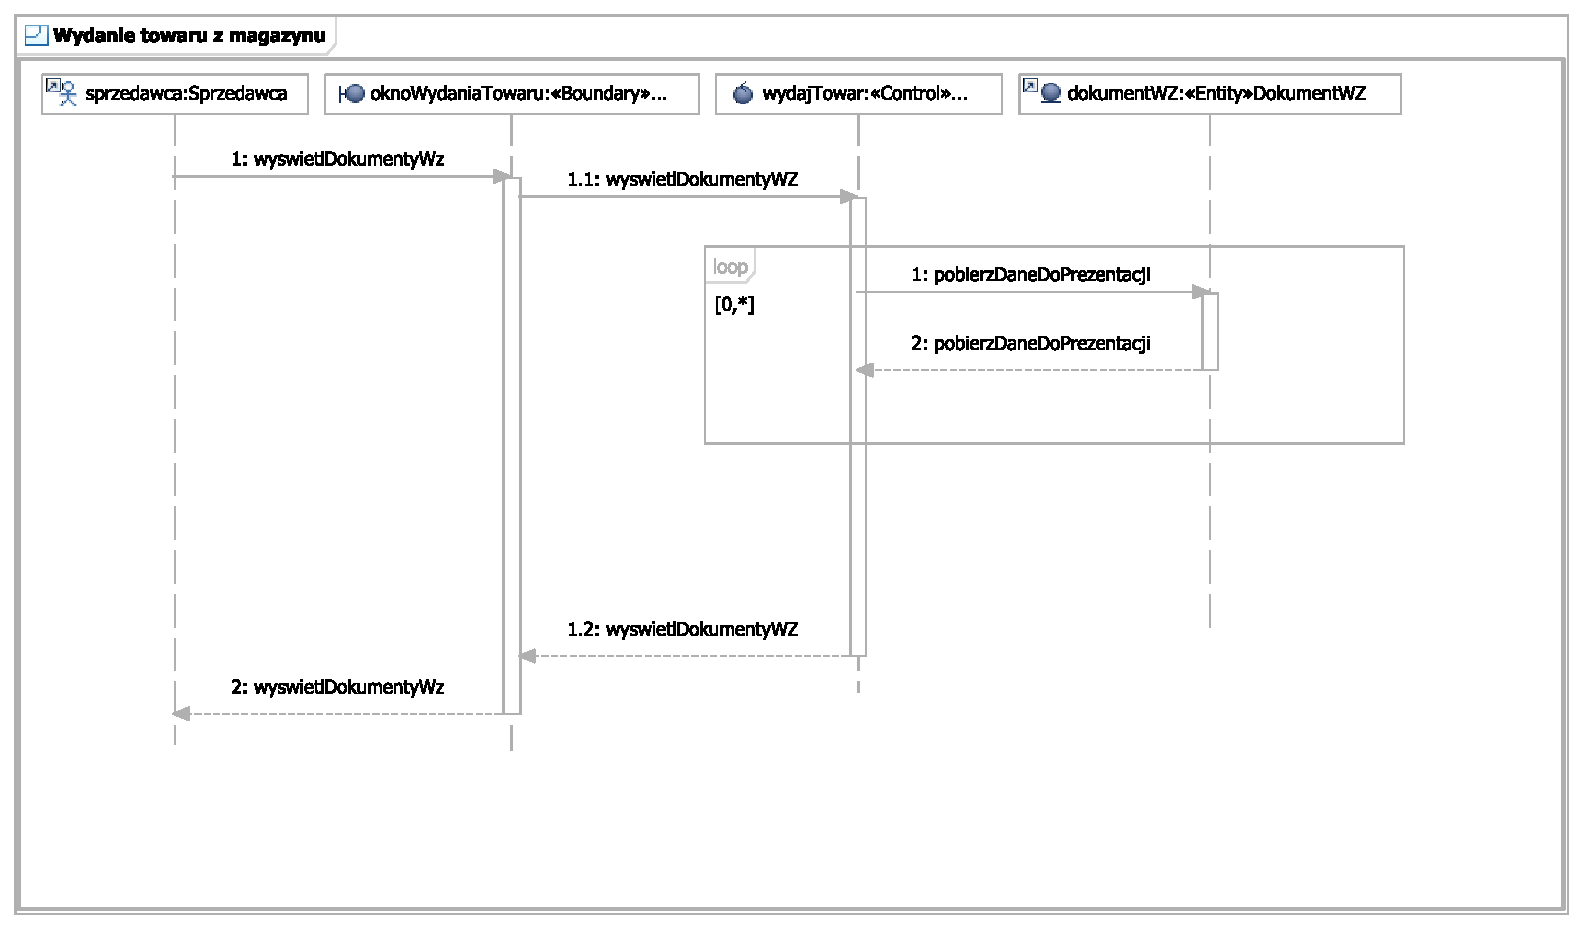
\includegraphics[angle=\seqangle, scale=\seqscale]{../img/usecase/pu12seq.pdf}
  \caption{\seqcaption12}
\end{figure}
\newpage

\subsection{Tworzenie dokumentu wydania towaru}
\begin{usecase}
  \addtitle{PU13}{Tworzenie dokumentu wydania towaru}
  \addfield{Priorytet:}{wysoki}
  \addfield{Aktor główny:}{Sprzedawca}
  \addfield{Rozszerza przypadki:}{PU12}
  \addfield{Warunki początkowe:}{Aktor został uwierzytelniony.}
  \additemizedfield{Warunki końcowe:}{ 
    \item Dokument wydania towaru został zapisany w systemie.
    \item Aktor otrzymuje informacje o poprawnym dodaniu dokumentu do systemu.
    \item Użytkownik może wyświetlić dokument na liście dokumentów wydania towaru. 
    \item Ilość przechowywanego towaru została zaktualizowana o ilość towaru zapisanego w dokumencie wydania towaru.
    \item Ilość przechowywanego towaru jest zgodna z warunkami poprawności danych przedstawionymi w \ref{dziedzina-problemu}.
  }
  \addscenario{Scenariusz główny:}{
    \item Aktor wybiera opcję utworzenia nowego dokumentu wydania towaru.
    \item System wyświetla formularz nowego dokumentu wydania towaru.
    \item Aktor wypełnia podstawowe dane dokumentu.
    \item Aktor wybiera kontrahenta operacji.
    \item Aktor wybiera towary, które będą wydane kontrahentowi.
    \item Aktor wskazuje ilość oraz cenę jednostkową wydawanego towaru.
    \item Aktor wybiera opcję zapisania dokumentu.
    \item System informuje aktora, że dane zostały poprawnie zaktualizowane.
  }
  \addscenario{Scenariusz alternatywny:} {
    \item [3.a] Aktor nie podał wymaganych pól formularza:
      \begin{enumerate}
        \item[1--4.] Jak w scenariuszu głównym.
        \item[5.] System wyświetla powiadomienie o konieczności podania wymaganych informacji.
        \item[6.] Aktor wraca do punktu 3.  
      \end{enumerate}
    \item [3.b] Aktor podał błędne wartości pól formularza:
      \begin{enumerate}
        \item[1--4.] Jak w scenariuszu głównym.
        \item[5.] System wyświetla powiadomienie o błędnych polach formularza.
        \item[6.] Aktor wraca do punktu 3.
      \end{enumerate}
     \item[5.a] Aktor wybrał ten sam towar co najmniej dwa razy.
       \begin{enumerate}
       \item[1--5.] Jak w scenariuszu głównym.
       \item[6.] System informuje aktora, że co najmniej dwa razy wybrał ten sam towar, podane ilości towaru zostaną więc zsumowane.
       \item[7.] System wyświetla zsumowane wartości dla tych samych towarów.
       \item[8--...] Jak w scenariuszu głównym.
       \end{enumerate}
  }
  \addfield{Zakres przetwarzanych danych:} {
    Pola dokumentu wydania towaru takie jak przedstawione w rozdziale \ref{dziedzina-problemu}.
  }
  \addfield{Warunki poprawności danych:}{
    Warunki poprawności takie jak przedstawione w rozdziale \ref{dziedzina-problemu}.
  }
  \addfield{Wymagania funkcjonalne:}{5.1}
\end{usecase}

\begin{figure}[H]
  \centering
  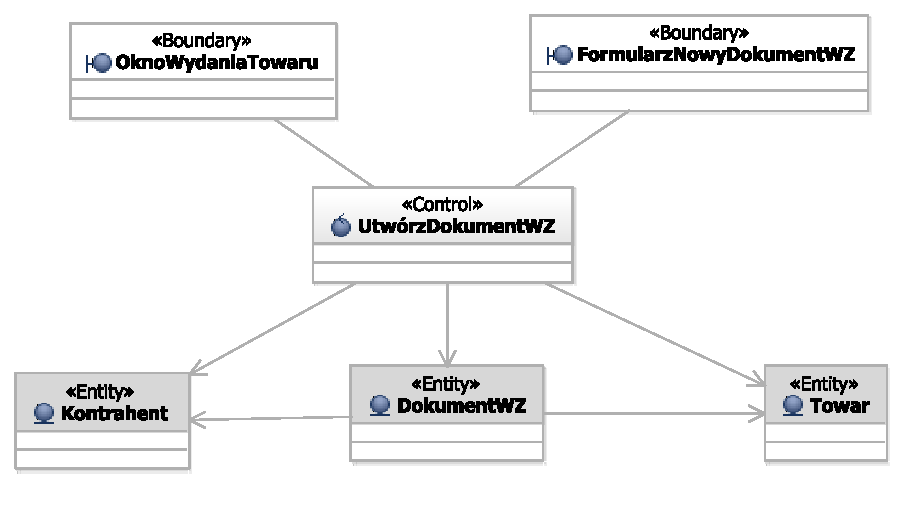
\includegraphics[angle=\ecbangle, scale=\ecbscale]{../img/usecase/pu13ecb.pdf}
  \caption{\ecbcaption13}
\end{figure}
\newpage
\begin{figure}[H]
  \centering
  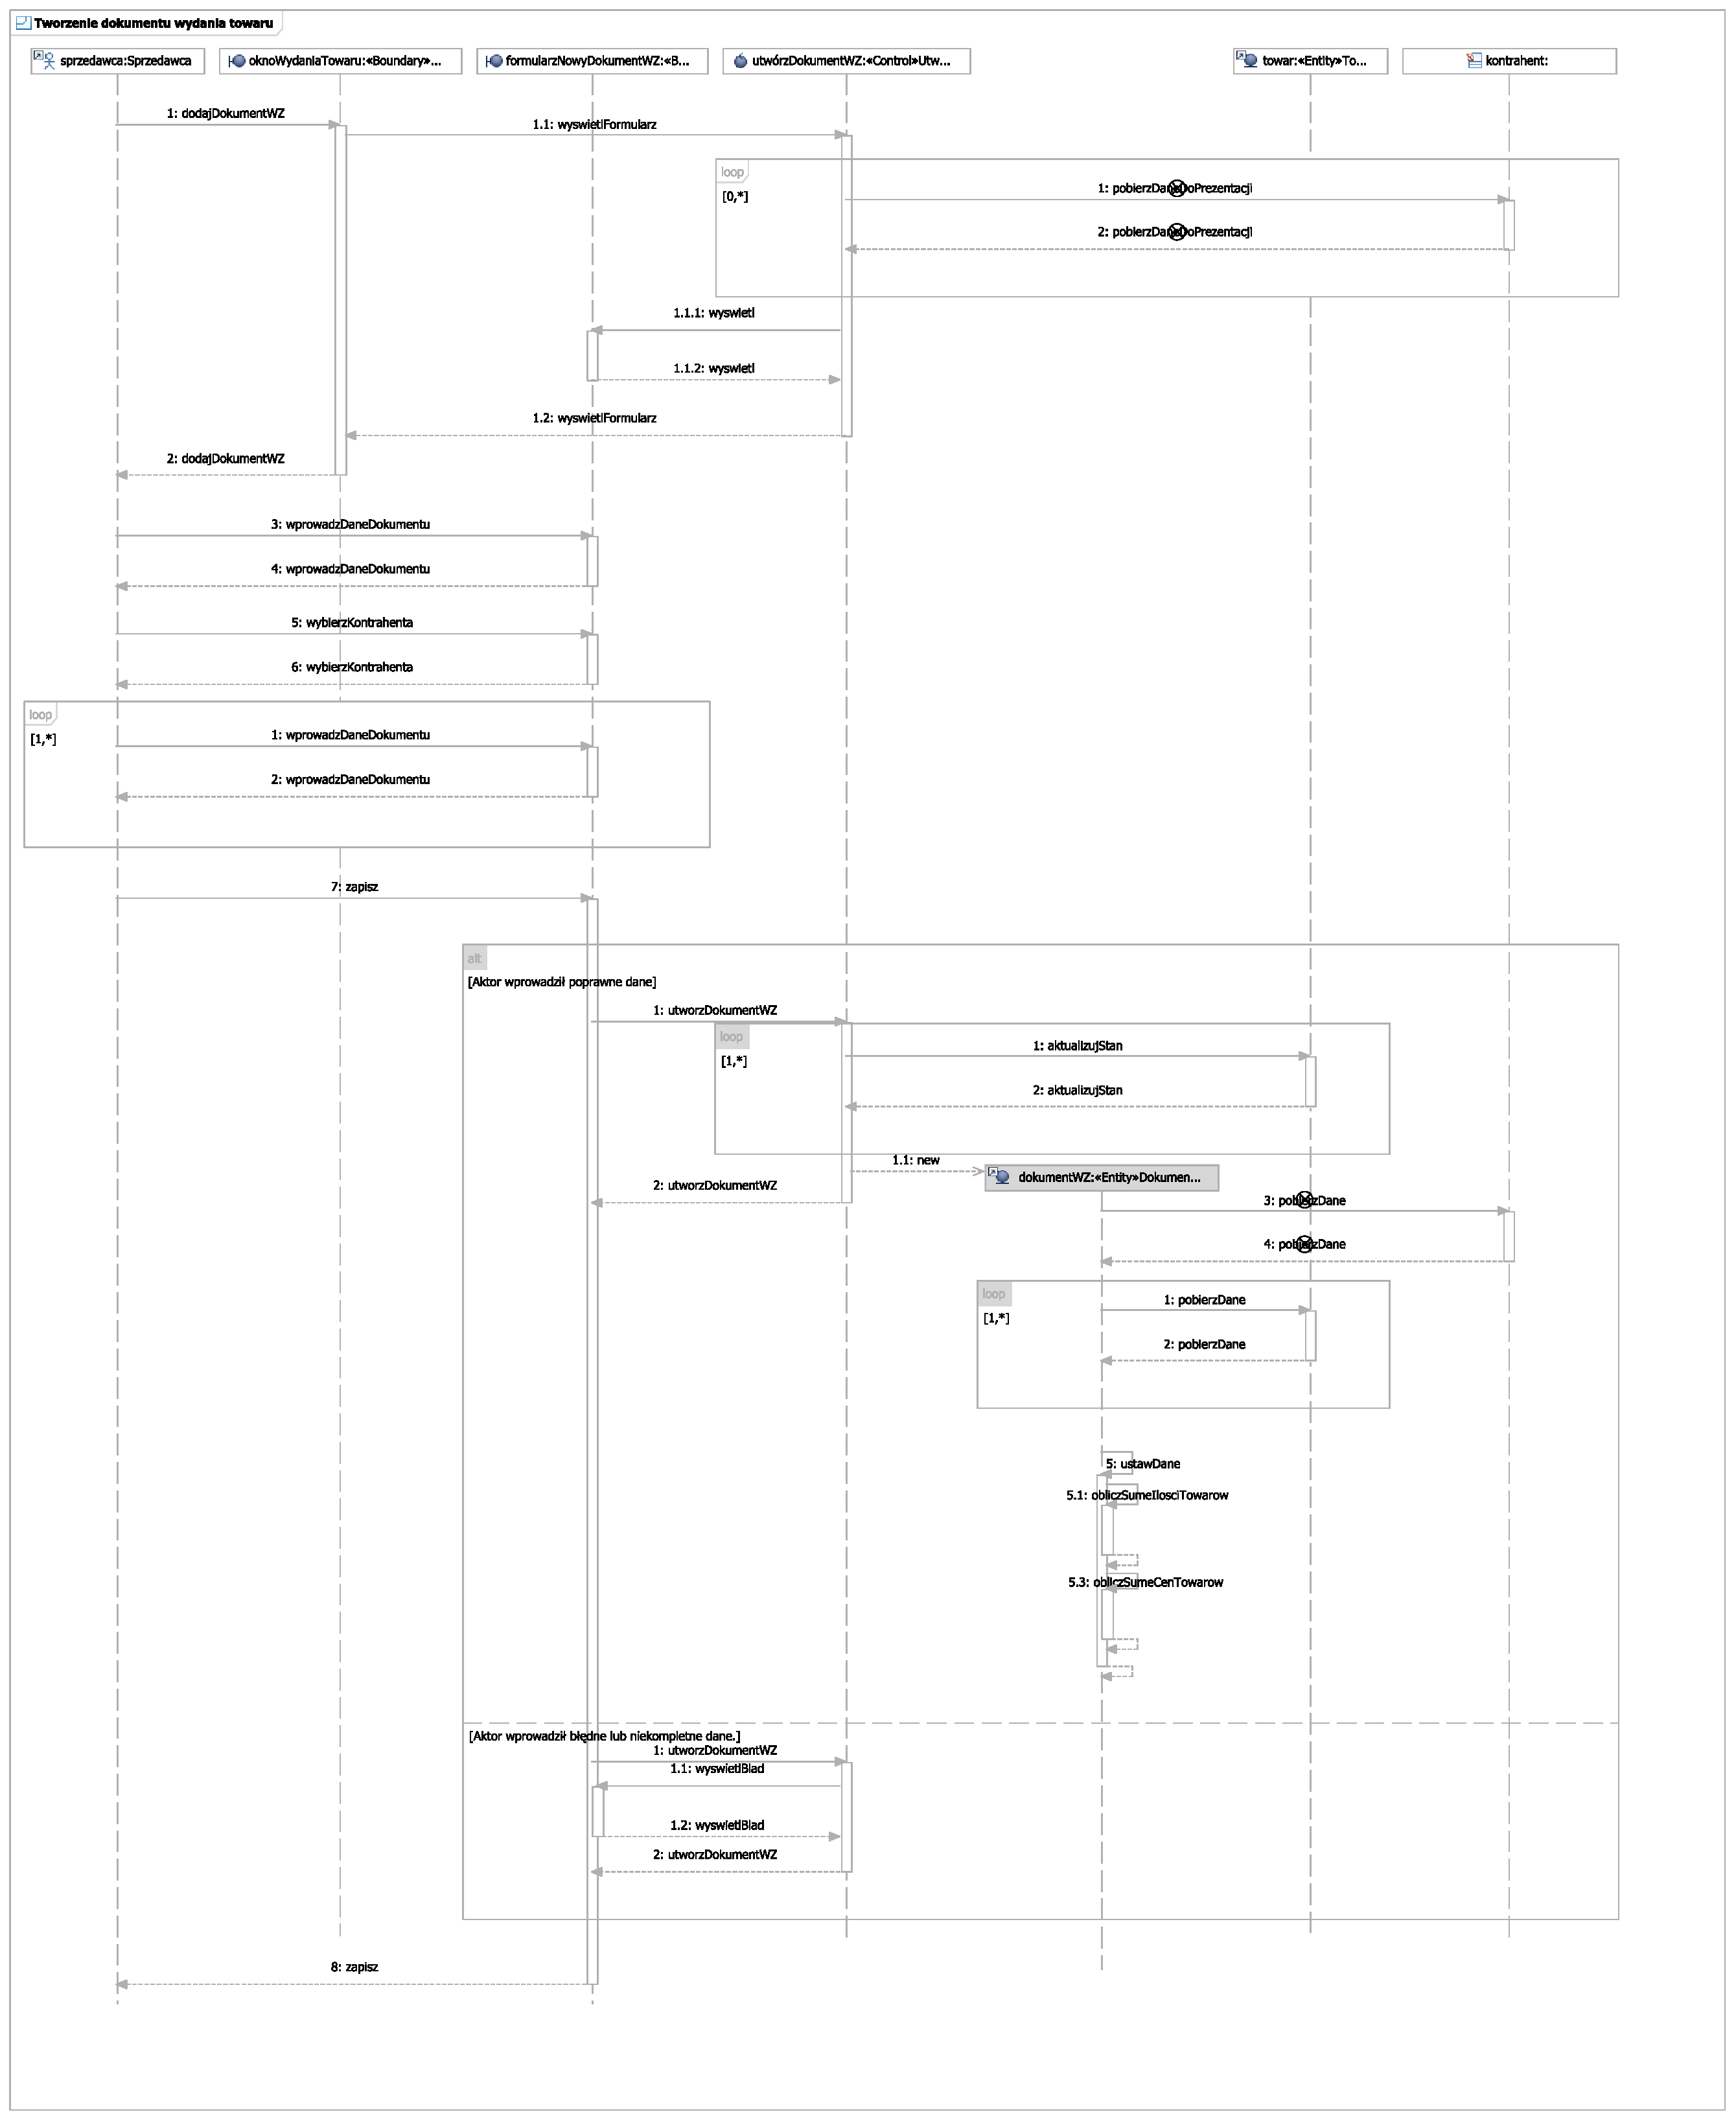
\includegraphics[angle=\seqangle, scale=0.35]{../img/usecase/pu13seq.pdf}
  \caption{\seqcaption13}
\end{figure}
\newpage

\subsection{Edycja dokumentu wydania towaru}
\begin{usecase}
  \addtitle{PU14}{Edycja dokumentu wydania towaru}
  \addfield{Priorytet:}{wysoki}
  \addfield{Aktor główny:}{Sprzedawca}
  \addfield{Rozszerza przypadki:}{PU12}
  \additemizedfield{Warunki początkowe:}{
    \item Aktor został uwierzytelniony.
    \item Operacja wydania towaru, którego dotyczy wybrany dokument, nie została jeszcze zrealizowana.
  }
  \additemizedfield{Warunki końcowe:}{ 
    \item Dane dokumentu zostały zaktualizowane w systemie.
    \item Aktor otrzymuje informację o poprawnej aktualizacji dokumentu.
    \item Użytkownik może wyświetlić dane dokumentu na liście dokumentów wydania towaru. 
    \item Ilość przechowywanego towaru została zaktualizowana o ilość towaru zapisanego w dokumencie wydania towaru.
    \item Ilość przechowywanego towaru jest zgodna z warunkami poprawności danych przedstawionymi w \ref{dziedzina-problemu}.
  }
  \addscenario{Scenariusz główny:}{
    \item Aktor wybiera opcję edycji wybranego dokumentu wydania towaru.
    \item System wyświetla formularz edycji dokumentu wydania towaru.
    \item Aktor wypełnia podstawowe dane dokumentu (oprócz pól wykluczonych z edycji).
    \item Aktor aktualizuje listę towarów, ich ilości oraz ceny jednostkowe.
    \item Aktor wybiera opcję aktualizacji dokumentu.
    \item System informuje aktora, że dane zostały poprawnie zaktualizowane.
  }
  \addscenario{Scenariusz alternatywny:} {
    \item [3.a] Aktor nie podał wymaganych pól formularza:
      \begin{enumerate}
        \item[1--4.] Jak w scenariuszu głównym.
        \item[5.] System wyświetla powiadomienie o konieczności podania wymaganych informacji.
        \item[6.] Aktor wraca do punktu 3.  
      \end{enumerate}
    \item [3.b] Aktor podał błędne wartości pól formularza:
      \begin{enumerate}
        \item[1--4.] Jak w scenariuszu głównym.
        \item[5.] System wyświetla powiadomienie o błędnych polach formularza.
        \item[6.] Aktor wraca do punktu 3.
      \end{enumerate}
     \item[4.a] Aktor wybrał ten sam towar co najmniej dwa razy.
       \begin{enumerate}
       \item[1--4.] Jak w scenariuszu głównym.
       \item[5.] System informuje aktora, że co najmniej dwa razy wybrał ten sam towar, podane ilości towaru zostaną więc zsumowane.
       \item[6.] System wyświetla zsumowane wartości dla tych samych towarów.
       \item[7--...] Jak w scenariuszu głównym.
       \end{enumerate}
  }
  \addfield{Zakres przetwarzanych danych:} {
    Pola dokumentu wydania towaru takie jak przedstawione w rozdziale \ref{dziedzina-problemu}.
  }
  \addfield{Warunki poprawności danych:}{
    Warunki poprawności takie jak przedstawione w rozdziale \ref{dziedzina-problemu}.
  }
  \addfield{Wymagania funkcjonalne:}{5.2}
\end{usecase}

\begin{figure}[H]
  \centering
  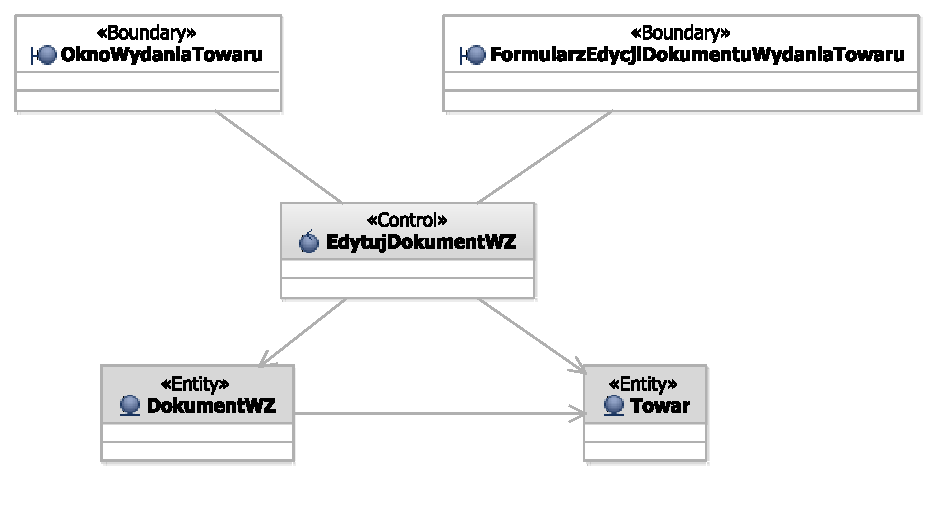
\includegraphics[angle=\ecbangle, scale=\ecbscale]{../img/usecase/pu14ecb.pdf}
  \caption{\ecbcaption14}
\end{figure}
\newpage
\begin{figure}[H]
  \centering
  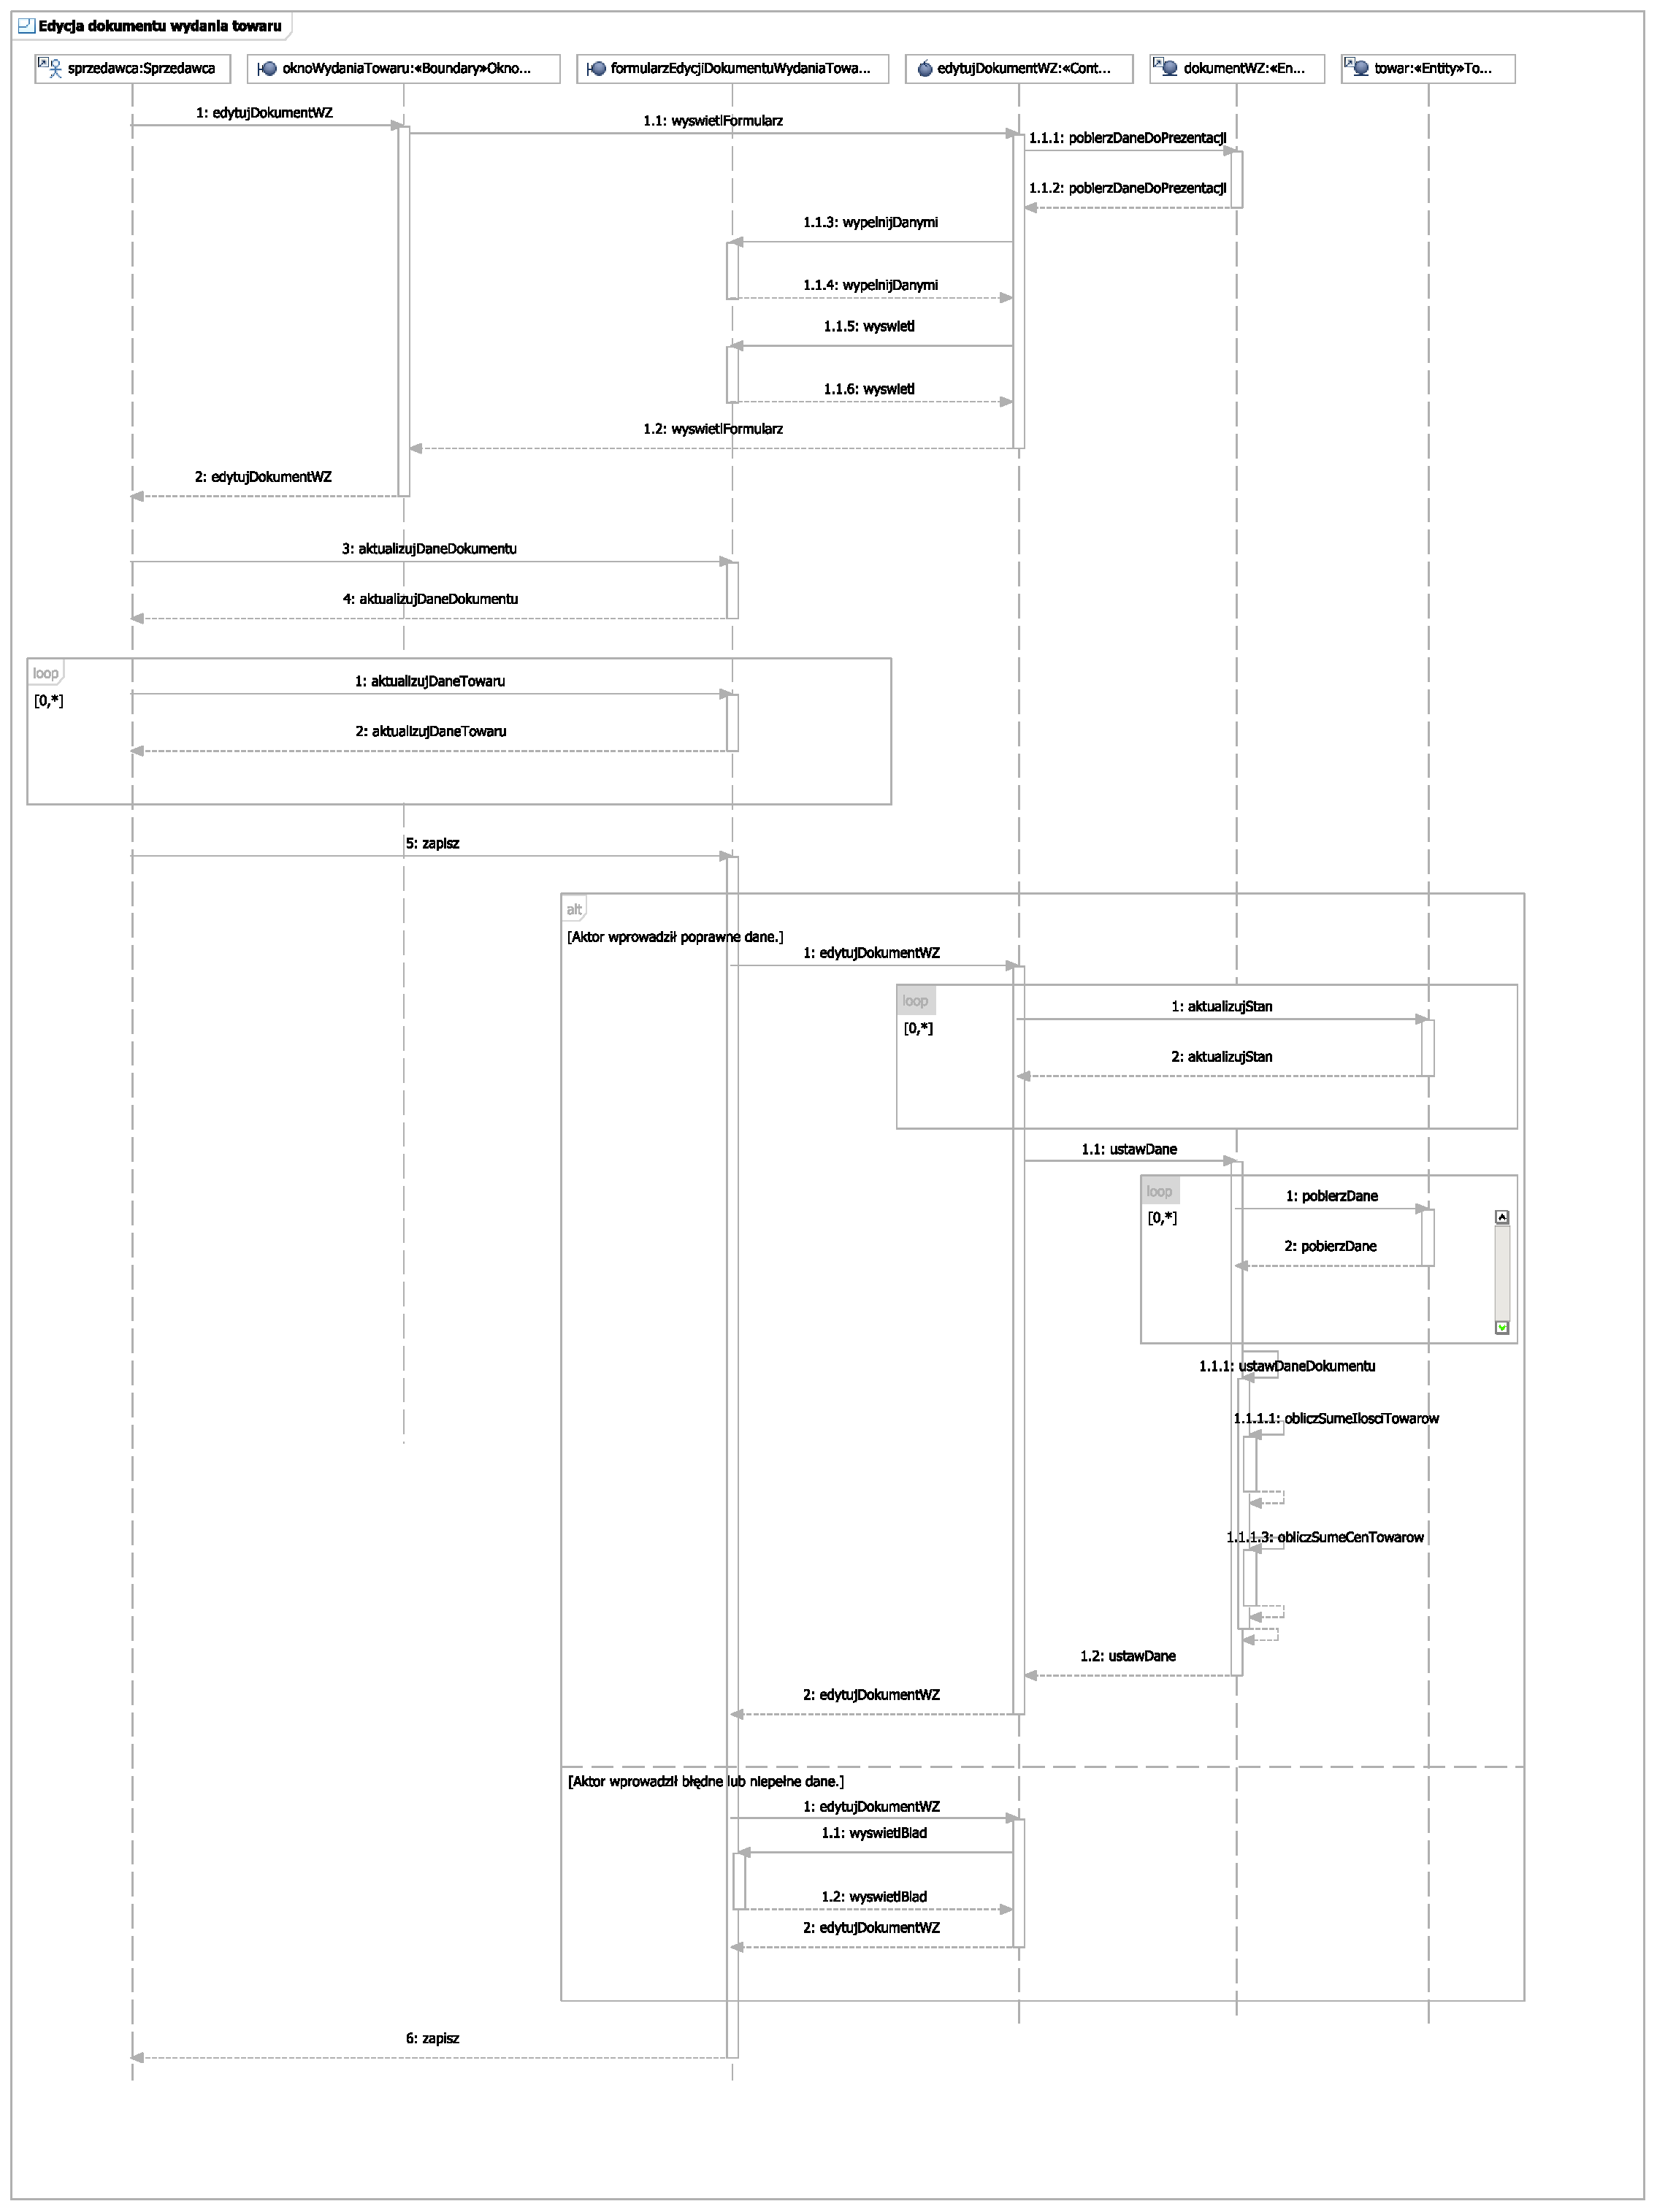
\includegraphics[angle=\seqangle, scale=\seqscalemin]{../img/usecase/pu14seq.pdf}
  \caption{\seqcaption14}
\end{figure}
\newpage

\subsection{Usuwanie dokumentu wydania towaru}
\begin{usecase}
  \addtitle{PU15}{Usuwanie dokumentu wydania towaru}
  \addfield{Priorytet:}{wysoki}
  \addfield{Aktor główny:}{Sprzedawca}
  \addfield{Rozszerza przypadki:}{PU12}
  \addfield{Warunki początkowe:}{Aktor został uwierzytelniony.}
  \additemizedfield{Warunki końcowe:}{
    \item Dane dokumentu zostały usunięte z systemu.
    \item Usunięty dokument nie jest wyświetlany na liście dokumentów wydania towaru.
    \item Stan towarów z usuniętego dokumentu jest zaktualizowany o ilości zapisane w usuwanym dokumencie.
  }
  \addscenario{Scenariusz główny:}{
    \item Aktor wybiera opcję usunięcia dokumentu wydania towaru z systemu.
    \item System prosi o potwierdzenie operacji.
    \item Aktor potwierdza usunięcie dokumentu z systemu.
    \item System wyświetla informację o pomyślnym usunięciu dokumentu z systemu.
  }
  \addscenario{Scenariusz alternatywny:}{
    \item[2.a] Aktor anuluje usunięcie dokumentu z systemu.
      \begin{enumerate}
        \item[1.--2.] Jak w scenariuszu głównym.
        \item[3.] Aktor anuluje usunięcie dokumentu z systemu.
        \item[4.] System wyświetla informację, że operacja została anulowana.
      \end{enumerate}
  }
  \addfield{Wymagania funkcjonalne:}{5.3}
\end{usecase}

\begin{figure}[H]
  \centering
  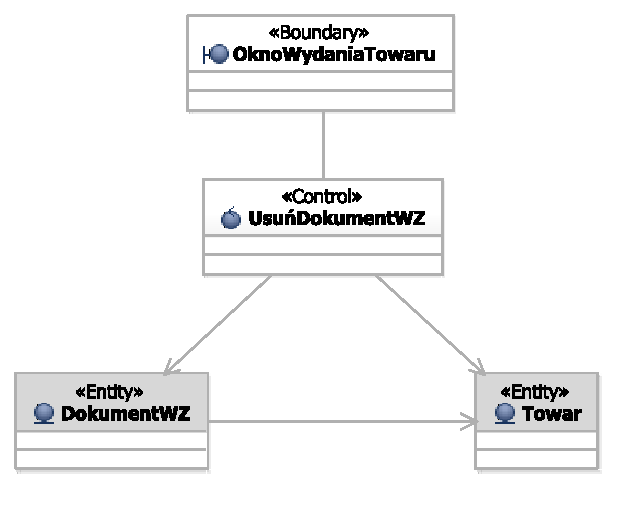
\includegraphics[angle=\ecbangle, scale=\ecbscale]{../img/usecase/pu15ecb.pdf}
  \caption{\ecbcaption15}
\end{figure}

\begin{figure}[H]
  \centering
  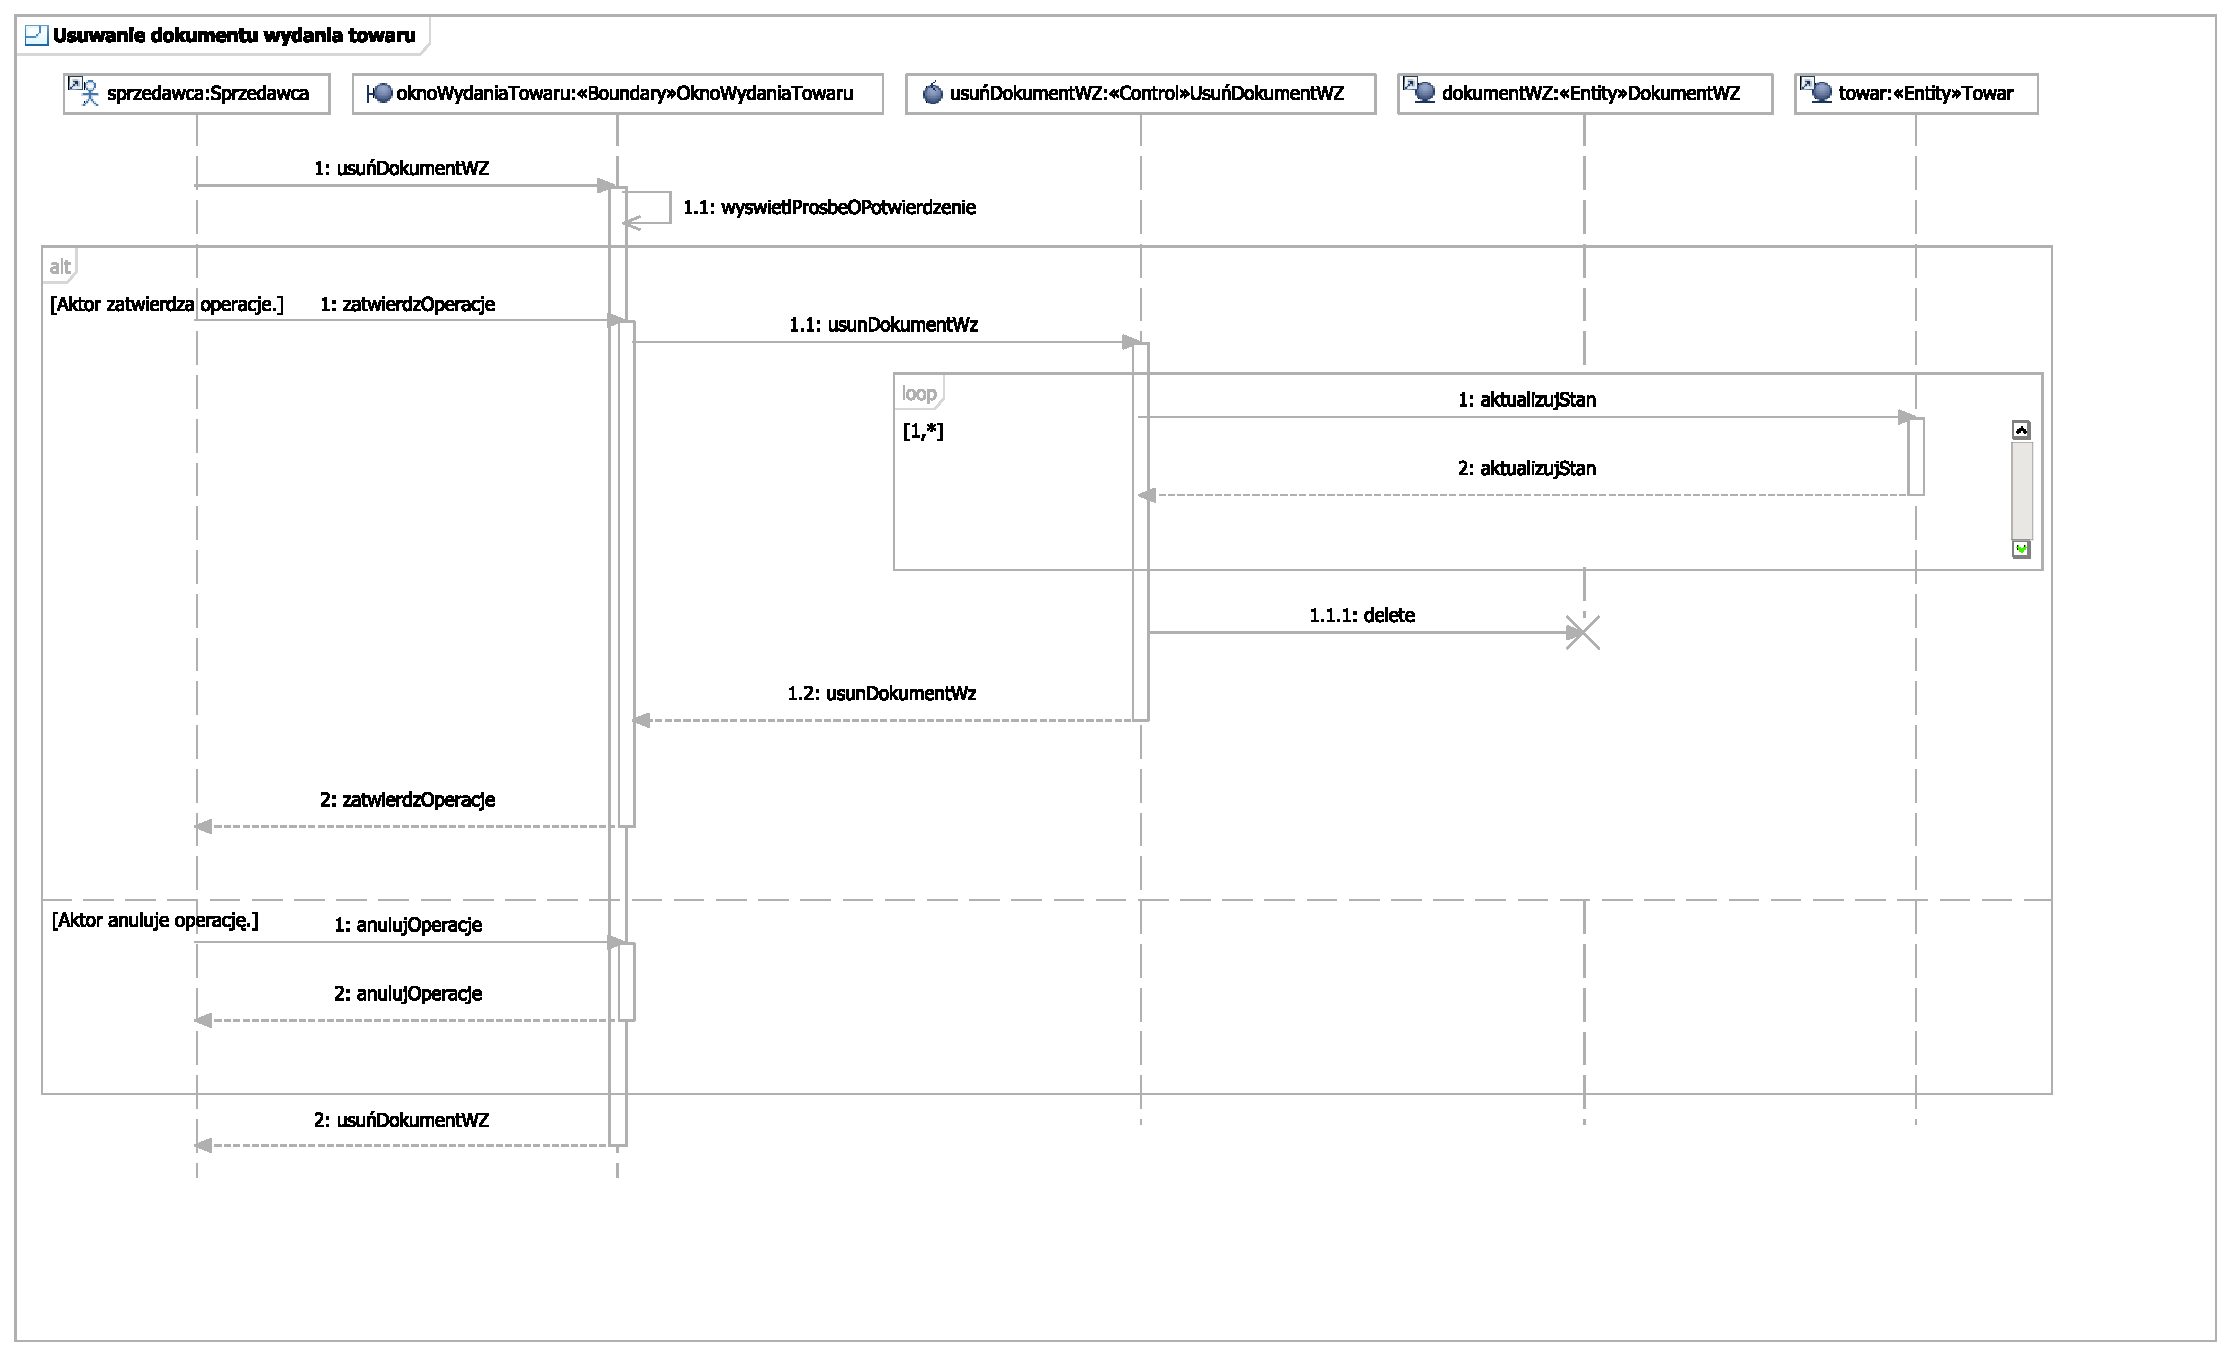
\includegraphics[angle=\seqangle, scale=0.42]{../img/usecase/pu15seq.pdf}
  \caption{\seqcaption15}
\end{figure}
\newpage

\subsection{Realizacja wydania towaru z magazynu}
\begin{usecase}
  \addtitle{PU16}{Realizacja wydania towaru z magazynu}
  \addfield{Priorytet:}{wysoki}
  \addfield{Aktor główny:}{Sprzedawca}
  \addfield{Rozszerza przypadki:}{PU12}
  \additemizedfield{Warunki początkowe:}{
    \item Aktor został uwierzytelniony.
    \item Wybrane wydanie towaru nie zostało jeszcze zrealizowane.}
  \additemizedfield{Warunki końcowe:} {
    \item Dokument wydania towaru został oznaczony jako zrealizowany.
    \item Możliwe jest utworzenie korekty do zrealizowanego dokumentu wydania towaru.
  }
  \addscenario{Scenariusz główny:}{
     \item Aktor wybiera opcję wydania towaru z magazynu.
     \item System prosi o potwierdzenie realizacji wydania towaru z magazynu.
     \item Aktor potwierdza realizację wydania towaru z magazynu.
     \item System oznacza dokument wydania towaru jako zrealizowany.
  }
 \addscenario{Scenariusz alternatywny:}{
    \item[4.a] Aktor anuluje realizację wydania towaru.
      \begin{enumerate}
        \item[1.--2.] Jak w scenariuszu głównym.
        \item[3.] Aktor anuluje realizację dokumentu.
        \item[4.] System wyświetla informację, że operacja została anulowana.
      \end{enumerate}
  }
  \addfield{Wymagania funkcjonalne:}{5.4}
\end{usecase}

\begin{figure}[H]
  \centering
  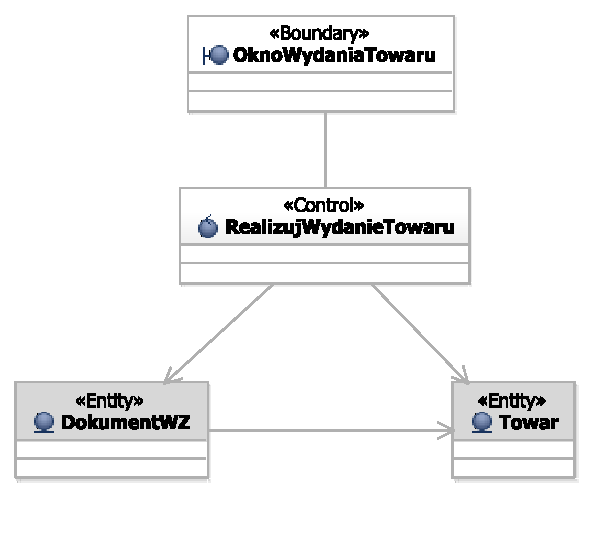
\includegraphics[angle=\ecbangle, scale=\ecbscale]{../img/usecase/pu16ecb.pdf}
  \caption{\ecbcaption16}
\end{figure}

\begin{figure}[H]
  \centering
  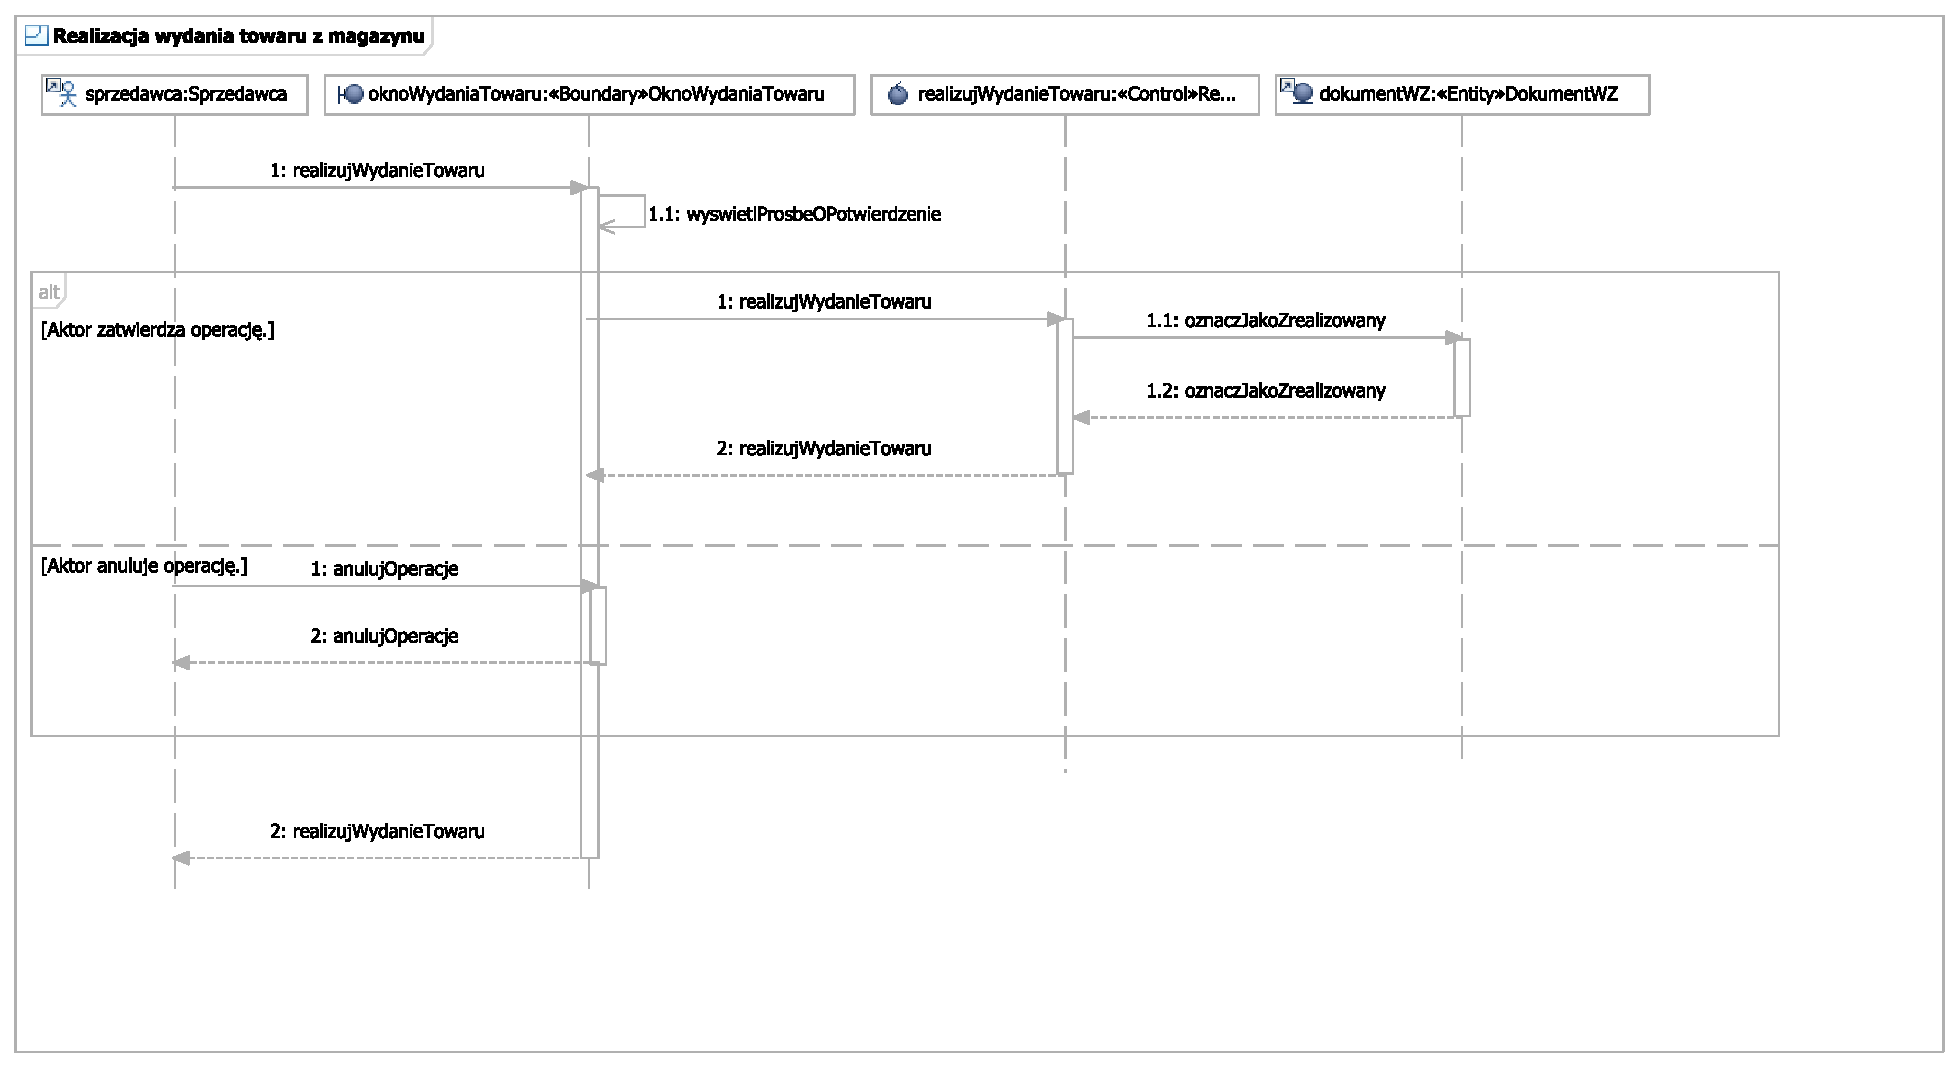
\includegraphics[angle=\seqangle, scale=0.5]{../img/usecase/pu16seq.pdf}
  \caption{\seqcaption16}
\end{figure}
\newpage

\subsection{Korekta wydania towaru}
\begin{usecase}
  \addtitle{PU17}{Korekta wydania towaru}
  \addfield{Priorytet:}{wysoki}
  \addfield{Aktor główny:}{Sprzedawca}
  \addfield{Rozszerza przypadki:}{PU12, PU13}
  \additemizedfield{Warunki początkowe:}{
     \item Aktor został uwierzytelniony.
     \item Wybrany dokument wydania towaru został już zrealizowany.
  }
  \additemizedfield{Warunki końcowe:}{ 
    \item Dokument korekty wydania towaru został zapisany w systemie.
    \item Ilość przechowywanych towarów została zaktualizowana zgodnie z wartością podaną na korekcie. 
    \item Ilość przechowywanego towaru jest zgodna z warunkami poprawności danych przedstawionymi w \ref{dziedzina-problemu}.
  }
  \addscenario{Scenariusz główny:}{
    \item Aktor wybiera opcję utworzenia korekty dla wskazanego dokumentu przyjęcia towaru.
    \item System wyświetla formularz nowej korekty. 
    \item Aktor wypełnia podstawowe dane korekty.
    \item Aktor wybiera towary, które podlegają zwrotowi oraz ich cenę.
    \item Aktor wybiera opcję zapisania korekty.
    \item System informuje aktora, że dane zostały poprawnie zaktualizowane.
  }
  \addscenario{Scenariusz alternatywny:} {
    \item [3.a] Aktor nie podał wymaganych pól formularza:
      \begin{enumerate}
        \item[1--4.] Jak w scenariuszu głównym.
        \item[5.] System wyświetla powiadomienie o konieczności podania wymaganych informacji.
        \item[6.] Aktor wraca do punktu 3.  
      \end{enumerate}
    \item [3.b] Aktor podał błędne wartości pól formularza:
      \begin{enumerate}
        \item[1--4.] Jak w scenariuszu głównym.
        \item[5.] System wyświetla powiadomienie o błędnych polach formularza.
        \item[6.] Aktor wraca do punktu 3.
      \end{enumerate}
     \item[5.a] Aktor wybrał ten sam towar co najmniej dwa razy.
       \begin{enumerate}
       \item[1--5.] Jak w scenariuszu głównym.
       \item[6.] System informuje aktora, że co najmniej dwa razy wybrał ten sam towar, podane ilości towaru zostaną więc zsumowane.
       \item[7.] System wyświetla zsumowane wartości dla tych samych towarów.
       \item[8--...] Jak w scenariuszu głównym.
       \end{enumerate}
  }
  \addfield{Zakres przetwarzanych danych:} {
    Pola dokumentu wydania towaru takie jak przedstawione w rozdziale \ref{dziedzina-problemu}.
  }
  \addfield{Warunki poprawności danych:}{
    Warunki poprawności takie jak przedstawione w rozdziale \ref{dziedzina-problemu}.
  }
  \addfield{Wymagania funkcjonalne:}{5.5}
\end{usecase}

\begin{figure}[H]
  \centering
  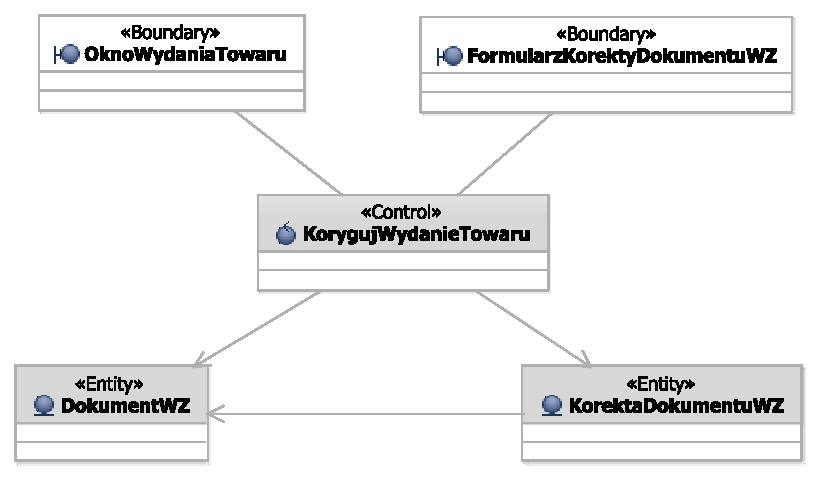
\includegraphics[angle=\ecbangle, scale=\ecbscale]{../img/usecase/pu17ecb.pdf}
  \caption{\ecbcaption17}
\end{figure}
\newpage
\begin{figure}[H]
  \centering
  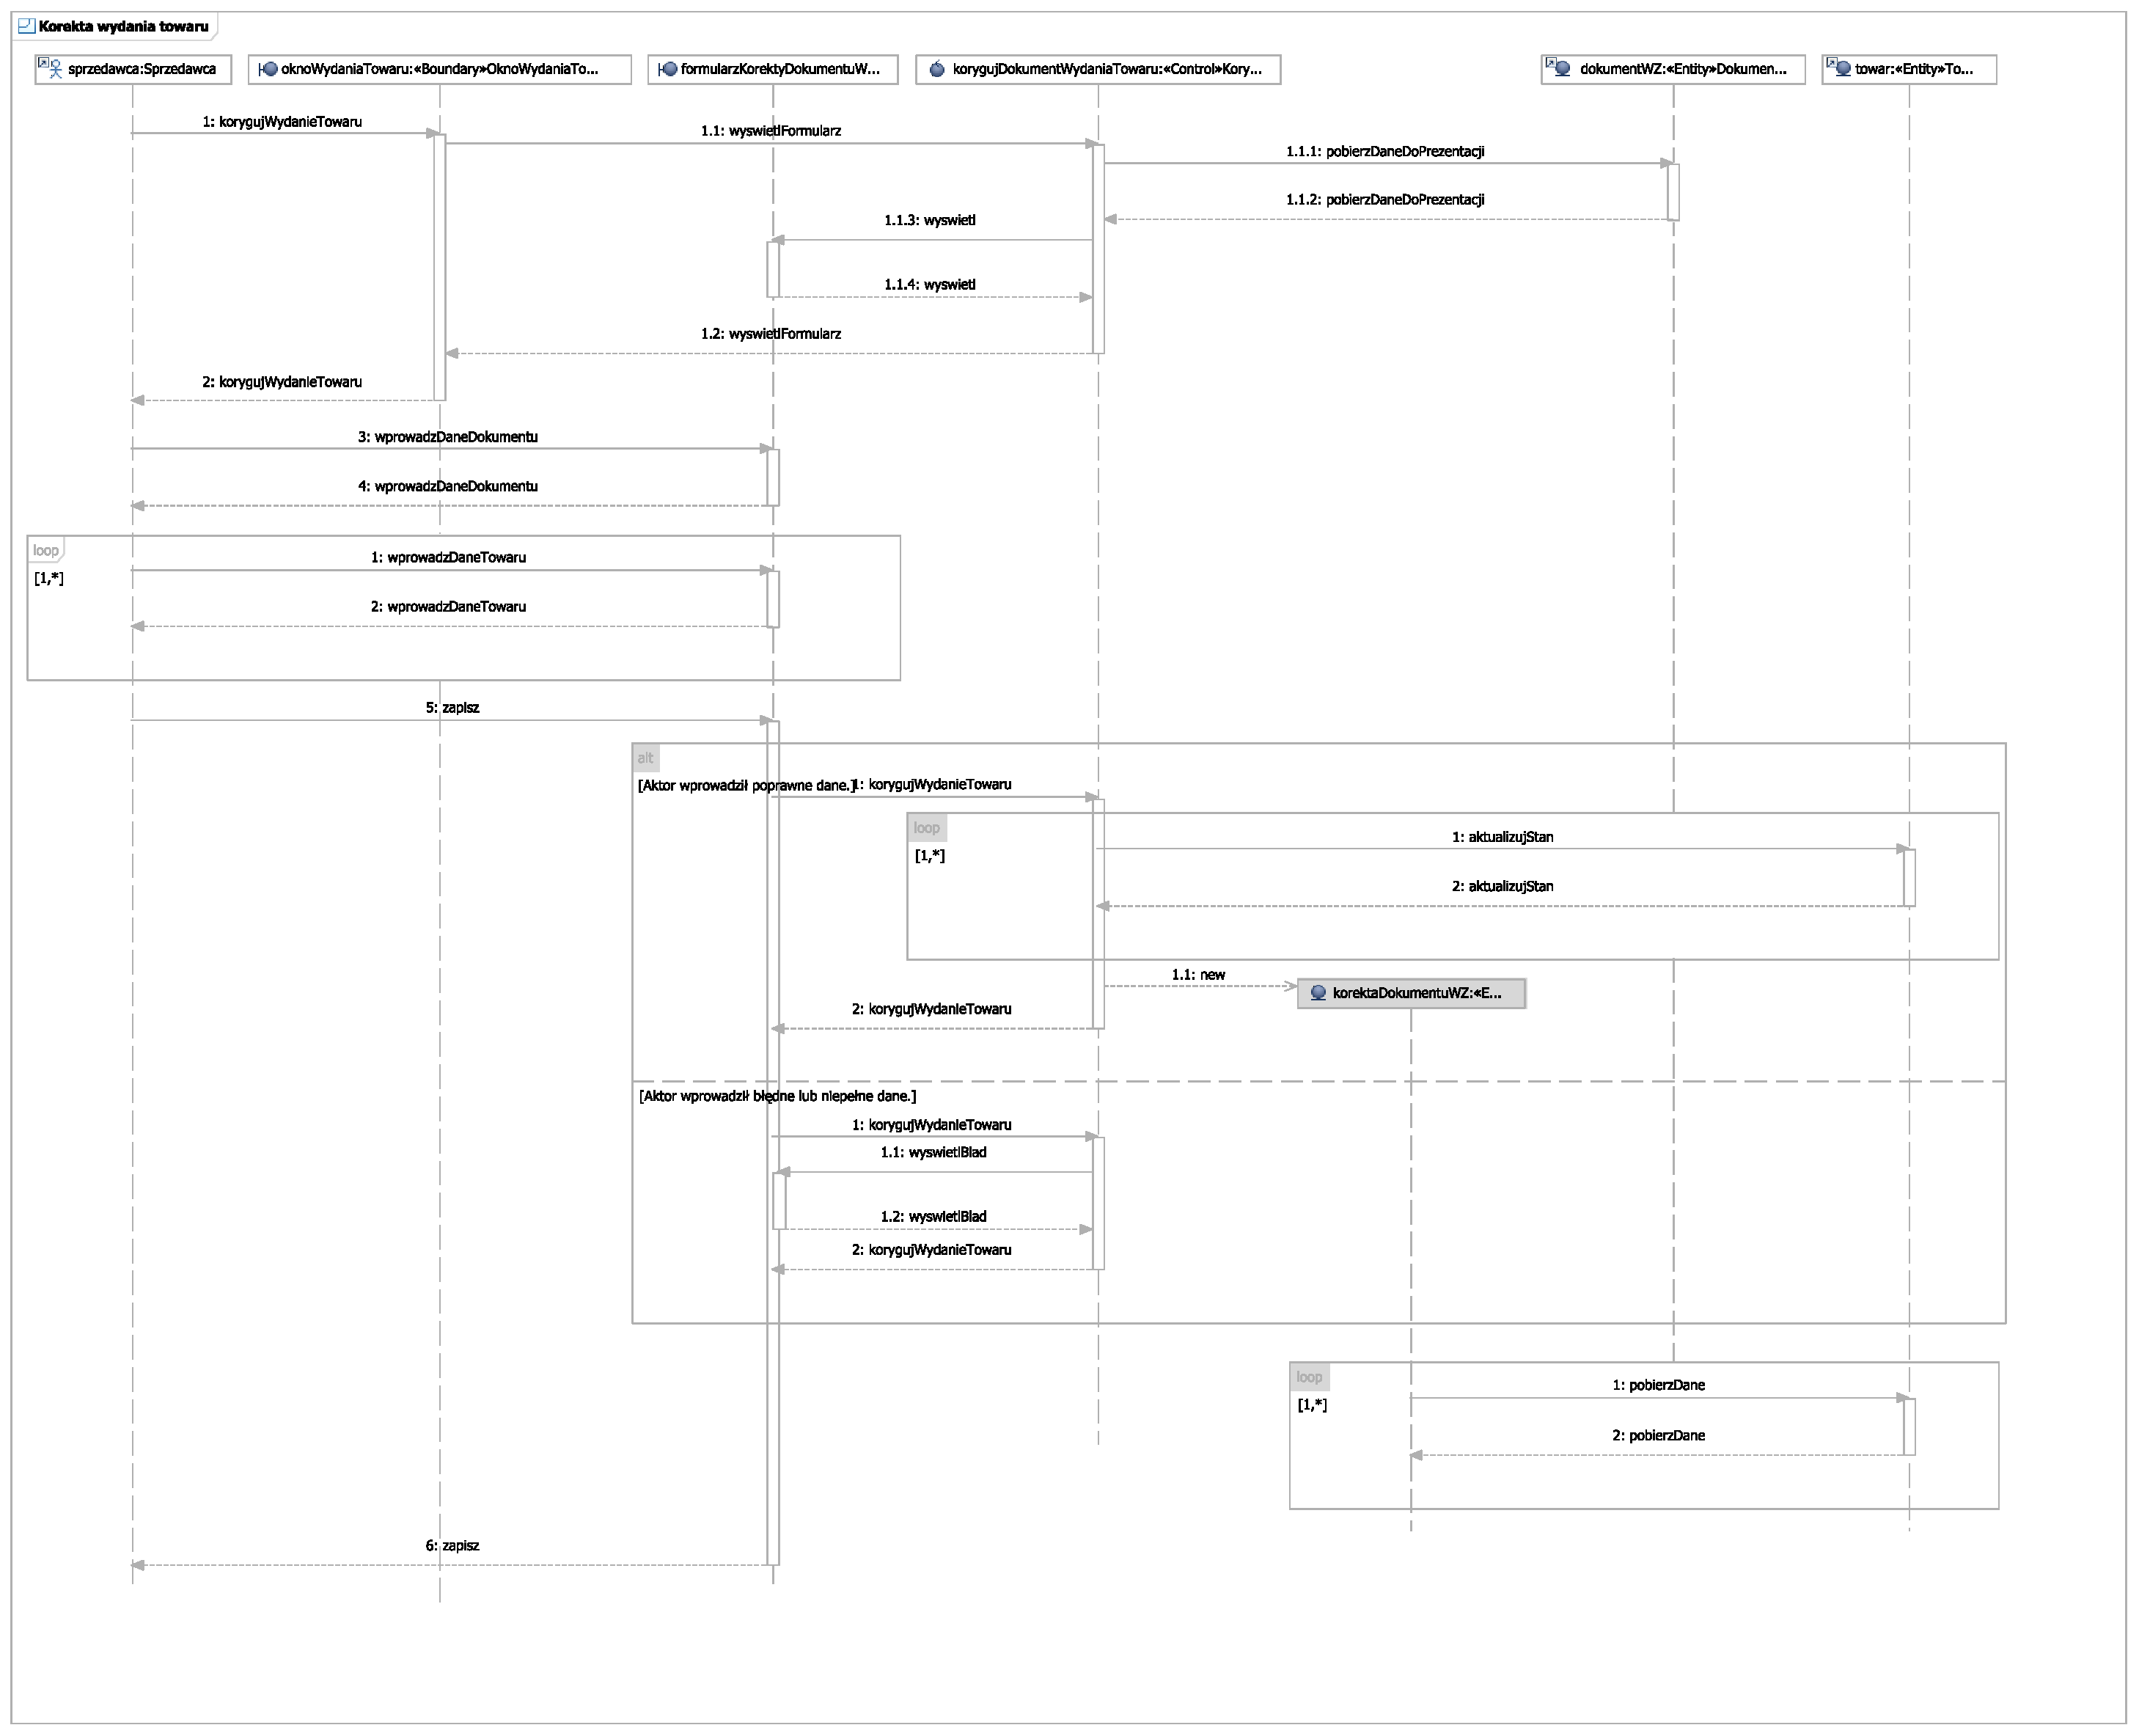
\includegraphics[angle=\seqangle, scale=0.32]{../img/usecase/pu17seq.pdf}
  \caption{\seqcaption17}
\end{figure}
\newpage





